% !TEX encoding = UTF-8 Unicode
% !TEX encoding = UTF-8 Unicode
\documentclass[12pt, a4paper]{article}
\pagestyle{headings}

\usepackage[brazil]{babel}
\usepackage[utf8]{inputenc}
\usepackage[T1]{fontenc}
\usepackage{textcomp}

\usepackage{amssymb, amsmath, pxfonts}

\usepackage{verbatim}
\usepackage{graphicx}
\usepackage{latexsym}
\usepackage{mathrsfs}

\usepackage{indentfirst}										% Adds tabs automatically

\usepackage[normalem]{ulem}										% Underlines words
\usepackage[top=3cm,left=3cm,right=3cm,bottom=3cm]{geometry}	% Margins

\usepackage[usenames]{color}									% Colored letters
\usepackage{makeidx}											% To create the index

\expandafter\def\expandafter\normalsize\expandafter{%
    \normalsize
    \setlength\abovedisplayskip{2pt}
    \setlength\belowdisplayskip{12pt}
    \setlength\abovedisplayshortskip{2pt}
    \setlength\belowdisplayshortskip{12pt}
}

\newcommand{\ui}{\mathrm{i}}
\newcommand{\ud}{\mathrm{d}}

\author{Cássio dos Santos Sousa}
\title{Elipses e Órbitas Planetárias}

\begin{document}

\maketitle

\tableofcontents

\newpage

\section{Introduction}

Muitos dos conceitos relacionados a órbitas e à Gravitação require basic knowledge about ellipses. It will be shown here two ways to analyse an ellipse mathematically: first using its equation in Cartesian coordinates, and second using its equation in polar coordinates. After that, the main analyses involving Gravitation will be made, linking the concepts of ellipses to describe planetary orbits.

\section{Definition}

The ellipse , by definition , is the locus of points the sum of whose distances from two fixed points is constant. The trajectory described by this locus is closed, and resembles a circle. The degenerated ellipse (in which these two points coincide) is indeed the circumference. It is one of the most known and used conics.

\section{Nomenclature}

A simple drawing of the ellipse to be analyzed is one in which, in Cartesian coordinates, the line determined by fixed points (named \textbf{major axis}) is aligned with the \textit{x}-  or \textit{y}-axis (Fig. 1).

\begin{figure}[!htb]
    \centering
     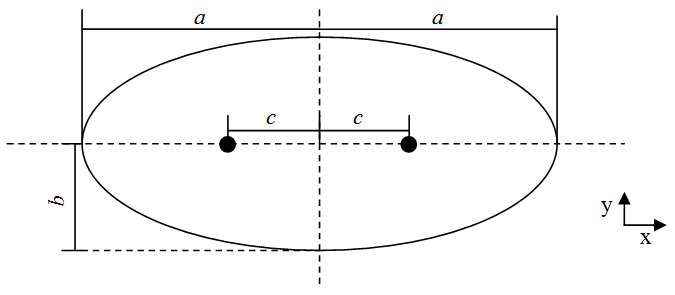
\includegraphics[scale=0.5]{elipse0.png}
    {\emph{\caption{Ellipse drawing with the x-axis aligned with the major axis.}}}
	\label{fig1}
\end{figure}

A nomenclatura relevante às seções seguintes é dada a seguir. Outros termos relevantes terão seções próprias para serem mostrados e definidos apropriadamente.

\begin{itemize}
    \item{\textbf{Focos:} pontos fixos (destacados em preto) que desenham a elipse;}
    \item{\textbf{Distância focal (2c):} distância entre os focos;}
    \item{\textbf{Semi-eixo maior (a):} distância entre o centro e o ponto mais distante da elipse;}
    \item{\textbf{Semi-eixo menor (b):} distância entre o centro e o ponto mais próximo da elipse.}
    \item{\textbf{Eixo principal/secundário:} contém o semi-eixo maior/menor.}
\end{itemize}

Frente à essa nomenclatura, é fácil de perceber que a soma das distâncias da definição é igual à \textbf{2a}. Basta considerar os pontos da elipse no eixo principal: a soma das distâncias é (a-c)+(a+c) = 2a. E usaremos isso para deduzir a equação da elipse.

\section{Equação da elipse na forma cartesiana}

A forma mais simples de se enxergar a elipse em coordenadas cartesianas é dada na fig. 1. Tomando estes eixos como base, deduziremos a equação da elipse para um ponto (x,y) qualquer dela, colocando o centro da elipse na origem do sistema de coordenadas (fig. 2). Será utilizada geometria básica para isso.

\begin{figure}[!htb]
    \centering
     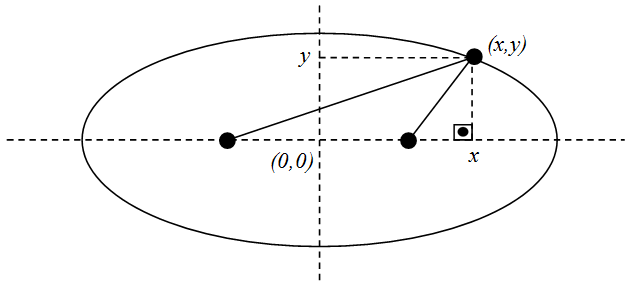
\includegraphics[scale=0.5]{elipse2.png}
    {\emph{\caption{Esquema de uma elipse com um ponto (x,y) destacado.}}}
    \label{fig2}
\end{figure}

Dada a definição e o Teorema de Pitágoras, podemos chegar que:
\begin{eqnarray}
    \sqrt{y^2 + (x-c)^2} + \sqrt{y^2 + (x+c)^2} = 2a \label{eq1}
\end{eqnarray}

Vamos então elevar ambas as expressões ao quadrado, isolando termos semelhantes e raízes, até chegar na expressão final:

\[
	\lim_{x \rightarrow a}{f(x)} = L
\]

\[
	\left(\sqrt{y^2 + (x-c)^2} + \sqrt{y^2 + (x+c)^2}\right) = (2a)^2 
\]
\[
	2y^2+ 2x^2 + 2c^2 + 2\sqrt{\left(y^2+(x-c)^2\right)\left(y^2+(x+c)^2\right)} = 4a^2  \\
\]
\[
	\left(y^2+(x-c)^2\right)\left(y^2+(x+c)^2\right) = (2a^2 - y^2 - x^2 - c^2)^2 \\
\]
\[
	0 = 4a^4 - 4a^2y^2 - 4a^2x^2 - 4a^2c^2 + 4x^2c^2 \\
\]
\[ 
	a^2(a^2-c^2) = x^2(a^2-c^2) + y^2a^2    
\]

As equações anteriores apenas desenvolveram a expressão (\ref{eq1}), tendo em mente que as raízes precisavam sumir da expressão inicial e que termos semelhantes precisavam ser agrupados ou removidos, ou seja, o intuito era simplificar. Dividindo a última equação apresentada por $a^2(a^2 - c^2)$, chegaremos que:
\begin{eqnarray}
    \frac{x^2}{a^2} + \frac{y^2}{a^2 - c^2} = 1 \label{eq2}
\end{eqnarray}

Esta equação ainda não tem o formato conhecido por muitas pessoas. Usemos então as definições para uma equação mais simples, usando o semi-eixo menor \textit{b} (fig. 3). {\\}

\begin{figure}[!htb]
    \centering
     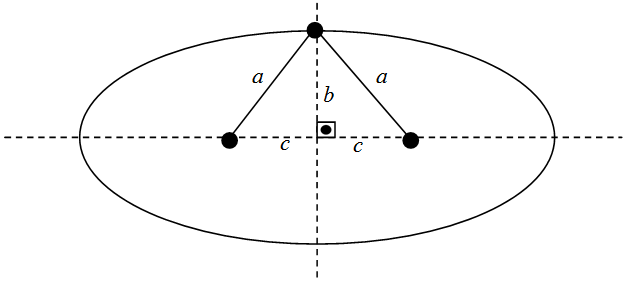
\includegraphics[scale=0.5]{elipse3.png}
    {\emph{\caption{Ponto notável de elipse, mostrando o semi-eixo menor.}}}
    \label{fig3}
\end{figure}

Pela definição, a soma das distâncias do foco aos pontos da elipse é constante. Tomemos então o ponto mais próximo do centro, que é denotado pelo semi-eixo menor. Como as distâncias aos focos são iguais, ambas valem \textit{a}. Dado o triângulo retângulo da figura acima, pelo Teorema de Pitágoras:
\begin{eqnarray}
    a^2 = b^2 + c^2 \label{eq3}
\end{eqnarray}

Utilizando a equação (\ref{eq3}) na equação (\ref{eq2}), chegamos então que:
\begin{eqnarray}
   \bf{\frac{x^2}{a^2} + \frac{y^2}{b^2} = 1} \label{eq4}
\end{eqnarray}

Esta é a \textbf{equação da elipse em coordenadas cartesianas} que tão bem conhecemos. Há um outro formato conhecido da equação da elipse, no qual o centro da elipse está presente num ponto $(x_0, y_0)$, fora da origem. A prova é deixada ao leitor, mas o formato e a prova da equação seguinte são bem semelhantes ao da equação (\ref{eq4}):

\begin{eqnarray}
    \frac{(x-x_0)^2}{a^2} + \frac{(y-y_0)^2}{b^2} = 1 \label{eq5}
\end{eqnarray}

Há também um útlimo formato da equação da elipse cartesiana, o qual considera o formato rotacionado dos eixos. No entanto, para a Gravitação, ele nos será pouco útil, uma vez que as coordenadas mais utilizadas são as polares. Mas antes de mostrarmos a elipse em coordenadas polares, utilizaremos uma medida muito comum em equações de cônicas, o \textit{semi-latus rectum} (ou \textit{semilatus rectum}), denotado pela letra \textit{l}.

\section{Semi-latus rectum}

O \textit{semi-latus rectum}, por definição, é a meia corda que passa pelo foco de uma cônica, é perperndicular ao eixo principal e tem um de seus extremos na própria cônica. Utilizemos então esta definição para a elipse (fig. 4).

\begin{figure}[!htb]
    \centering
     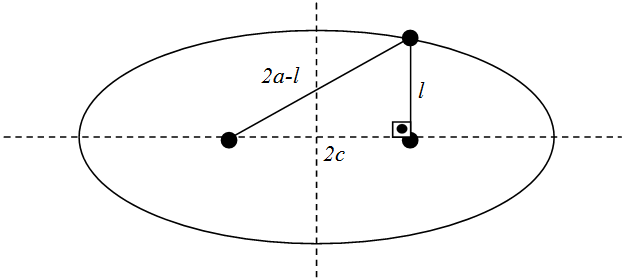
\includegraphics[scale=0.5]{elipse4.png}
    {\emph{\caption{Esquema utilizado para ilustrar o semi-latus rectum.}}}
    \label{fig4}
\end{figure}

Traçando a perpendicular recomendada, obtém-se uma corda de comprimento \textit{l}. Como esta corda é perpendicular, podemos utilizar este fato juntamente com a definição de elipse para descobrir o seu valor, por meio do Teorema de Pitágoras:

\begin{eqnarray}
	(2a-l)^2 = l^2 + 4c^2 \label{eq6}
\end{eqnarray}

Da equação anterior: {\\}
\[
	4a^2 - 4al = 4c^2
\]

\[
	 l = \frac{a^2 - c^2}{a}
\]

Da equação (\ref{eq3}):
\begin{eqnarray}
	\bf{l = \frac{b^2}{a}} \label{eq7}
\end{eqnarray}

\section{Excentricidade}

Algo também muito conhecido da Gravitação é a chamada \textbf{excentricidade}, muito comum no que se refere a órbitas. Pela definição, toda cônica pode ser definida como o lugar geométrico dos pontos cujas distâncias a um ponto e a uma reta possuem a mesma razão. No caso da elipse, há duas retas (uma para cada foco) externas e paralelas ao eixo secundário que possuem tal propriedade. Porém, tal definição não nos é útil. $\\$

Ao invés disso, utilizaremos uma outra definição: a excentricidade $\epsilon$ pode ser dada pela razão entre a excentricidade linear (definida como a distância entre o centro da cônica e qualquer um dos focos, neste caso \textit{c}) e o semi-eixo maior \textit{a}:
\begin{eqnarray}
	\epsilon = \frac{c}{a} \label{eq8}
\end{eqnarray}

Há formas diferentes de se enxergar \textit{c}, de acordo com a cônica avaliada. No caso da circunferência, os focos coincidem, então \textit{c} vale zero. No caso da parábola, ele coincide (em valor) com o semi-eixo maior. No caso da hipérbole, ele é maior que o semi-eixo maior, e o triângulo retângulo que contêm \textit{a}, \textit{b} e \textit{c} possui \textit{c} como hipotenusa. $\\$

Importar-nos-á, por enquanto, que a elipse possui $c<a$, e portanto $0<\epsilon <1$. Com estes valores definidos ($\epsilon$ e \textit{l}), podemos finalmente seguir à forma polar.

\section{Equação da elipse na forma polar}

Na forma polar, toma-se um dos focos como origem da distância radial \textit{r}, e a contagem do ângulo $\theta$ costuma começar a partir do eixo principal, no sentido anti-horário. Tomemos então um ponto qualquer da elipse definido pelo par $(r,\theta)$, e utilizaremos a definição de elipse para chegar na equação polar (fig. 5).

\begin{figure}[!htb]
    \centering
     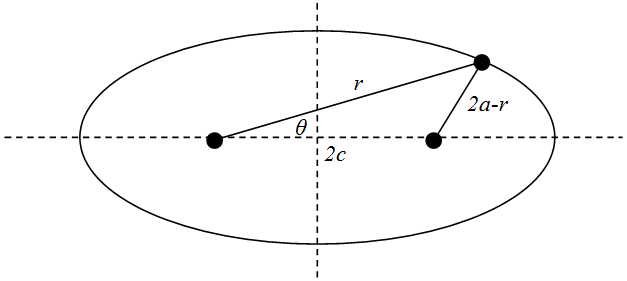
\includegraphics[scale=0.5]{elipse5.png}
    {\emph{\caption{Triângulo utilizado para se chegar na forma polar.}}}
    \label{fig5}
\end{figure}

Frente ao triângulo denotado acima, pela lei dos cossenos:

\begin{eqnarray}
	(2a-r)^2 = r^2 + (2c)^2 - 2(r)(2c)cos\theta \label{eq9}
\end{eqnarray}

Isolando \textit{r}:
\[
	a^2 - c^2 = r(a- ccos\theta)
\]

Dividindo tudo por \textit{a}:

\[
	\frac{a^2 - c^2}{a}= r\left(1- \left(\frac{c}{a}\right)cos\theta\right) \label{eq18}
\]{\\}

Com o auxílio das equações (\ref{eq7}) e (\ref{eq8}), podemos chegar à seguinte equação:

\begin{eqnarray}
	\bf{\frac{l}{r}=(1-\epsilon cos\theta)} \label{eq10}
\end{eqnarray}

A equação anterior é denominada \textbf{equação da elipse em coordenadas polares}. Há também um formato muito útil para o caso de elipses rotacionadas, pois ele não depende do alinhamento do eixo principal com outros eixos de referência:

\begin{eqnarray}
	\frac{l}{r}=(1-\epsilon cos(\theta - \theta_0)) \label{eq11}
\end{eqnarray}

As equações (\ref{eq10}) e (\ref{eq11}) podem ser utilizadas para representar qualquer cônica, definidos o \textit{semi-latus rectum} e a excentricidade. Estas mesmas equações são as bases da análise elíptica das equações de órbita na Gravitação.

\section{Forças centrais}

Entrando agora no âmbito da Gravitação propriamente dita, começaremos analisando as chamadas forças centrais. A definição formal de força central é a de que sua dependência é unicamente radial, i.e.:

\begin{eqnarray}
	\mathbf{F} =\mathbf{F}(\mathbf{r}) = F_r \mathbf{\hat{r}} \label{eq12}
\end{eqnarray}

Vendo a fórmula anterior de outra forma, ela nos traz que as componentes tangenciais (no caso de coordenadas esféricas, as componentes nas direções $\theta$ e $\phi$) são nulas em todo o espaço. E isso nos é muito útil, pois isso traz ótimas propriedades.

\subsection{Uma força central é conservativa}

Um detalhe muito bom da força central: o rotacional de \textbf{F} é \textbf{nulo}. {\\}

Para provar isso, basta utilizar a definição de rotacional para coordenadas esféricas:

\begin{eqnarray}
	\nabla \times \textbf{F} (r,\theta,\phi) = \frac{1}{r^2sen\theta} \begin{vmatrix} & \hat{r} &rsen\phi\hat{\theta} &  r\hat{\phi} & \\ \\ & \frac{\partial}{\partial r} & \frac{\partial}{\partial \theta} & \frac{\partial}{\partial \phi} & \\ \\ & F_r & rsen\phi F_{\theta} & rF_{\phi} & \end{vmatrix} \label{eq13}	
\end{eqnarray}

Desenvolvendo o determinante, com $F_{\theta}$ = $F_{\phi}$ = 0:

\[
	\nabla \times \textbf{F} (r,\theta,\phi) = \frac{1}{r}\left(\frac{\partial F_r}{\partial \phi}\right)\hat{\theta} - \frac{1}{rsen\phi}\left(\frac{\partial F_r}{\partial \theta}\right)\hat{\phi}
\]
{\\}

No entanto, $F_r$ depende apenas de \textbf{r}, então:

\begin{eqnarray}
	\nabla \times \mathbf{F} = \mathbf{0} \label{eq14}
\end{eqnarray}

Isso nos permite tirar a informação do enunciado. Para isso, é necessário avaliar uma outra equação, a fórmula de Stokes:

\begin{eqnarray}
	\oint_{\partial S} \mathbf{F}.\mathbf{dl} = \int_S (\mathbf{\nabla \times F}).\mathbf{dS}, \label{eq15}
\end{eqnarray}
sendo $S$ uma superfície \textit{qualquer} delimitada por um caminho fechado $\partial S$, e \textbf{dl} é um segmento de percurso feito ao longo de $\partial S$. No entanto, da equação (\ref{eq14}), o lado direito da equação de Stokes é sempre nulo. Logo, temos que, para uma força central:

\begin{eqnarray}
	\oint_{\partial S} \mathbf{F}.\mathbf{dl} = 0 \label{eq16}
\end{eqnarray}

A integral de uma força central ao longo de um percurso fechado \textit{qualquer} é nula. E isso nos será útil para descrever o que acontece com a energia potencial \textit{U} correspondente à força \textbf{F}, cuja relação infinitesimal, por definição, é trazida por:

\begin{eqnarray}
	dU= - \mathbf{F}.\mathbf{dl}  \label{eq17}
\end{eqnarray}

Se a força \textbf{F} é de fato conservativa, então a variação da energia potencial ao longo de um percurso fechado \textit{qualquer} tem de ser nulo (ou então a energia estaria sendo perdida em alguma outra forma). Se unirmos este conceito e as eqs. (\ref{eq16}) e (\ref{eq17}), chega-se que:

\begin{eqnarray}
	\oint_{\partial S} dU = 0, \label{eq18}
\end{eqnarray}
{\\}com $\partial S$ \textit{qualquer}. A expressão acima nos traz que \textbf{F} é conservativa.

\subsection{O momento angular é conservado}

Isso não tem muito a ver com o tópico anterior, pois a explicação pode ser dada em termos da própria trajetória do corpo sob ação da força \textbf{F}. {\\}

Considere a expressão do torque $\tau$ da força \textbf{F} num corpo que esteja a uma distância \textbf{r} em relação à origem do sistema radial definido para a força central:

\begin{eqnarray}
	\tau = \mathbf{r} \times \mathbf{F} \label{eq19}
\end{eqnarray}

Como \textbf{F} é central, então ele está na direção de \textbf{r}, o que nos traz:

\begin{eqnarray}
	\tau = \mathbf{r} \times (F_r\mathbf{\hat{r}}) = rF_r(\mathbf{\hat{r}} \times \mathbf{\hat{r}}) = \mathbf{0} \label{eq20}
\end{eqnarray}

O torque total da força é nulo, quaisquer que sejam a posição e a velocidade do corpo analisado (isso não é completamente válido para efeitos relativísticos, mas servirá bem para nosso propósito). Logo, o momento angular total é conservado.

\subsection{O movimento de um corpo devido a uma força central é plano}

Temos então que o momento angular \textbf{L} é constante. Se tomarmos a expressão original do momento angular:

\begin{eqnarray}
	\mathbf{L} = m\mathbf{r} \times \mathbf{v} \label{extra01}
\end{eqnarray}

Se \textbf{r} e \textbf{v} estiverem na mesma direção, o momento angular é nulo e o movimento está contido numa reta (pois a força é radial), a qual está contida não em um, mas em infinitos (mesmos) planos.{\\}

Se \textbf{r} e \textbf{v} não estiverem na mesma direção, eles nunca estarão na mesma direção que o momento angular. Primeiro, que o produto escalar entre \textbf{r} (ou \textbf{v}) e \textbf{L} será sempre nulo, uma vez que:
\begin{eqnarray}
	\mathbf{r.L} = m\mathbf{r}.(\mathbf{r} \times \mathbf{v}) \label{extra02}
\end{eqnarray}

A equação anterior determina um produto misto, que resulta em um escalar. Para vetores $\mathbf{a} = (a_1, a_2, a_3)$, $\mathbf{b} = (b_1, b_2, b_3)$ e $\mathbf{c} = (c_1, c_2, c_3)$, ele é dado por:

\begin{eqnarray}
	\mathbf{a . (b \times c)} = \begin{vmatrix} & a_1 & a_2 & a_3 &\\ \\&  b_1 & b_2 & b_3 &\\ \\ & c_1 & c_2 & c_3 &\end{vmatrix} \label{extra03}
\end{eqnarray} 

Como, no produto escalar de \textbf{r} (ou \textbf{v}) por \textbf{L}, haverá duas linhas iguais no determinante acima, ele será nulo. Se o produto escalar entre dois vetores é nulo, eles são perpendiculares entre si.{\\}

Como \textbf{L} é conservado, haverá  um plano que conterá a origem do sistema de coordenadas e será perpendicular ao momento angular (contendo, portanto, todos os vetores perpendiculares a ele). Logo, \textbf{r} e \textbf{v} (suficientes para descrever o movimento) estarão sempre contidos neste único plano (chamado também de \textbf{plano orbital}). 

\section{Força gravitacional}

A força gravitacional foi primeiramente descrita por Newton, e depois reavaliada por Einstein ao descrever a Relatividade Geral (procure por Mercúrio e sua peculiar "precessão de periélio" para ver a diferença). Mexerei apenas com alguns dizeres de Newton, o que já trará bastante trabalho e aprendizado por agora. {\\}

Sua análise veio da adoção de modelos para o movimento dos planetas. Como todos elas pareciam se mover de forma semelhante em torno de um mesmo corpo (o Sol) no céu, alguma (mesma) explicação precisava ser dada para descrever este movimento. Isso tudo (e mais outros detalhes) trouxeram à tona o formato particular da chamada \textbf{força gravitacional}, descrita pela equação (com K positivo):

\begin{eqnarray}
    \mathbf{F} = -\frac{K}{r^2}\mathbf{\hat{r}}    \label{eq21}
\end{eqnarray}

Esta equação chegou ao mundo de modo empírico, mas ela tem como base o formato de uma força atrativa (dado que os planetas se moviam em torno de órbitas fechadas, deveria haver uma resultante centrípeta - por isso o sinal negativo) e central (sendo o sistema heliocêntrico, o efeito deveria ter a mesma origem - o Sol). {\\}

Sendo uma força central, já sabemos que o movimento dos planetas é plano, o momento angular é conservado e a força é conservativa. Se transcrevermos estas quantidades por meio de equações apropriadas, encontraremos todas as propriedades de um movimento orbital. {\\}

Esta explicação pode ser estendida para qualquer movimento que tenha este mesmo formato para sua força de interação, como a interação eletrostática.

\section{Energia potencial gravitacional}

Detalhemos, primeiramente, o nosso K. Sendo a força essencialmente interativa, ela deveria depender de uma mesma propriedade dos corpos envolvidos. Newton propôs que esta propriedade seria a chamada \textit{massa gravitacional} (levemente diferente da chamada \textit{massa inercial} utilizada em $\mathbf{F} = m\mathbf{a}$, mas que, na prática, é bem próxima desta quantitativamente). Aqui chamaremos esse ente apenas de \textbf{massa}. {\\}

Faltaria ainda um fator de proporcionalidade. Ele é chamado de \textbf{constante universal da Gravitação}, ou apenas \textbf{constante gravitacional}, denotada por $G$. Unindo estes detalhes, podemos adequar a equação (\ref{eq21}) para nosso propósito:

\begin{eqnarray}
    \mathbf{F} = -\frac{GMm}{r^2}\mathbf{\hat{r}}    \label{eq22}
\end{eqnarray}

Nesta equação, $M$ denota a massa do corpo orbitado, $m$ denota a massa do corpo analisado, $r$ denota a distância entre os corpos, $\mathbf{\hat{r}}$ corresponde ao vetor unitário que parte do corpo orbitado para o corpo analisado, e:

\begin{eqnarray}
    G =  6,674287 \times 10^{-11}  m^3kg^{-1}s^{-2}   \label{eq23}
\end{eqnarray}

Como dito anteriormente, esta força é conservativa, então existe uma energia potencial associada a ela. Tomando esta energia por U(r) (não é necessária a notação vetorial, dado que so há dependência da posição e a força só atua radialmente), encontramos sua notação integrando a equação (\ref{eq17}):

\begin{eqnarray}
    U(r) - U(r_0) = -\int_{r_0}^{r}{\mathbf{F}.d\mathbf{r}}    \label{eq24}
\end{eqnarray}

Na equação anterior, $r_0$ é um valor de referência (posição na qual o potencial seria nulo). Dado que \textbf{F} depende inversamente do quadrado da distância \textit{r}, é de se esperar que corpos infinitamente distantes não interajam entre si, então tomar $r_0 \Rightarrow \infty$ nos servirá muito bem. Substituindo então a expressão de \textbf{F} na expressão anterior, temos:

\begin{eqnarray}
    U(r) - U(\infty) = -\int_{\infty}^{r}{\left(\frac{GMm}{r^2}\mathbf{\hat{r}}\right).\left(dr.\mathbf{\hat{r}}\right)} =  -GMm\int_{\infty}^{r}{\frac{dr}{r^2}}    \label{eq25}
\end{eqnarray}

Terminando a integração, tomando $U(\infty) = 0$, teremos que:

\begin{eqnarray}
    U(r) = -GMm\left(-\left.\frac{1}{r}\right|_{\infty}^r \right) = GMm \left( \frac{1}{\infty} - \frac{1}{r} \right)    \label{eq26}
\end{eqnarray}

Concluindo:

\begin{eqnarray}
    U(r) = -\frac{GMm}{r} \label{eq27}
\end{eqnarray}

É necessário verificar se $U(\infty) = 0$ de fato (isso foi uma consideração inicial). No entanto, como a distância \textit{r} está no denominador, é fácil perceber que esta relação procede. Sendo assim, a equação (\ref{eq27}) denota a \textbf{energia potencial gravitacional}.{\\}

Detalhada a energia potencial, podemos trabalhar em cima do momento angular e obter mais um termo de interesse. No entanto, estaremos entrando numa região no qual o movimento planetário será quase que unicamente abordado, então algumas considerações precisam ser feitas:

\section{Potencial efetivo}

A expressão tradicional da energia cinética é:

\begin{eqnarray}
    K = \frac{m}{2}\mathbf{v.v} \label{eq28}
\end{eqnarray}

Como o movimento de um corpo sob a força gravitacional é plano, é possivel descrevê-lo por meio de coordenadas polares (\textit{r, $\theta$}). Denotando a velocidade por meio deste novo eixo de coordenadas:

\begin{eqnarray}
   \mathbf{v} = \left(\frac{dr}{dt}\right)\mathbf{\hat{r}} + \left(r\frac{d\theta}{dt}\right)\mathbf{\hat{\theta}} \label{eq29}
\end{eqnarray}

Como $\mathbf{\hat{r}}$ e $\mathbf{\hat{\theta}}$ são ortogonais, podemos reescrever a expressão da equação (\ref{eq28}):

\begin{eqnarray}
    K = \frac{m}{2}\left[\left(\frac{dr}{dt}\right)^2 + r^2\left(\frac{d\theta}{dt}\right)^2\right] = \frac{m\dot{r}^2}{2} + \frac{mr^2\hat{\theta}^2}{2} \label{eq30}
\end{eqnarray}

No entanto, como já foi mencionado anteriormente, a força gravitacional não causa torque, o que nos traz que o momento angular \textbf{L} é constante. Se observarmos o movimento de um corpo orbitante, podemos aproximar seu Sol (ou corpo orbitado) para um corpo fixo (o erro, na prática, é pequeno). Para esta aproximação, podemos aproximar o módulo do momento angular para:
\begin{eqnarray}
    L = mr^2\dot{\theta} \label{eq31}
\end{eqnarray}

Utilizando a equação (\ref{eq31}) na equação (\ref{eq30}):

\begin{eqnarray}
    K = \frac{m\dot{r}^2}{2} + \frac{L^2}{2mr^2} \label{eq32}
\end{eqnarray}

Compilando então a energia total \textit{E}:

\begin{eqnarray}
    E = U + K = \frac{m\dot{r}^2}{2} + \mathbf{\frac{L^2}{2mr^2} - \frac{GMm}{r}} \label{eq33}
\end{eqnarray}

O termo destacado em negrito é chamado de \textbf{potencial efetivo, $\mathbf{V_{eff}}$}, e corresponde à parcela da energia que depende apenas da distância \textbf{r} envolvida:

\begin{eqnarray}
    V_{eff} = V_{eff}(r)  = \frac{L^2}{2mr^2} - \frac{GMm}{r} \label{eq34}
\end{eqnarray}

A análise gráfica desta função é muito interessante, pois ela traz uma forma muito interessante de se observar o movimento orbital. No entanto, este tema será retomado pouco tempo depois de ser apresentadas as definições de órbita, para que as coisas fiquem um pouco mais claras.

\section{Equação do movimento orbital}

Esta equação do movimento é trazida diretamente da expressão da energia mostrada na eq. (\ref{eq33}). No entanto, sua prova é razoavelmente longa, com varios termos e expressões pouco amigáveis a serem remanejadas. Ela será então mostrada em passos.

\subsection{1º passo: isolar tempo de distância}

Isolando a velocidade radial $\dot{r}$ na eq. (\ref{eq33}):

\[
	\frac{m\dot{r}^2}{2} = E - \frac{L^2}{2mr^2} + \frac{GMm}{r}
\]

\[
	 \dot{r} = \sqrt{\frac{2}{m}\left(E - \frac{L^2}{2mr^2} + \frac{GMm}{r}\right)}
\]

No entanto, como há uma derivada temporal envolvida:

\[
	\frac{dr}{dt} = \sqrt{\frac{2}{m}\left(E - \frac{L^2}{2mr^2} + \frac{GMm}{r}\right)}
\]

Da expressão acima, é possivel então isolar as variáveis \textit{r} e \textit{t}:

\begin{eqnarray}
	dt = \frac{dr}{\sqrt{\frac{2}{m}\left(E - \frac{L^2}{2mr^2} + \frac{GMm}{r}\right)}} \label{eq35}
\end{eqnarray}

\subsection{2º passo: mudanças de variável}

O tempo é uma variável muito interessante de se obter, pois é possivel então prever as varias posições da partícula. No entanto, a análise temporal de uma órbita não tem tanta informação quanto a descrição do movimento no plano orbital, do ponto de vista geométrico. Este movimento tem muito mais condições de contorno a serem avaliadas, e a análise temporal não nos trará isso com tanta clareza. {\\}

Ao invés de tempo, utilizaremos o ângulo $\theta$ definido da mesma forma que para o momento angular. Obteremos então uma equação de forma geral $r(\theta)$, em busca da avaliação do movimento como uma cônica. Isso é possível a partir da definição de momento angular, tomada na forma diferencial:

\[
	\frac{d\theta}{dt} = \frac{L}{mr^2}
\]

\begin{eqnarray}
	dt = \frac{mr^2}{L}d\theta \label{eq36}
\end{eqnarray}

Outra substituição que será muito útil, dados os expoentes envolvendo \textit{r} na equação (\ref{eq35}), será:

\begin{eqnarray}
	u = \frac{1}{r} \label{eq37}
\end{eqnarray}

A forma diferencial conveniente desta equação é:

\begin{eqnarray}
	du = -\frac{dr}{r^2} \label{eq38}
\end{eqnarray}

\subsection{3º passo: utilizando as novas variáveis}

Utilizando a equação (\ref{eq36}) na equação (\ref{eq35}):

\[
	\frac{mr^2}{L}d\theta = \frac{dr}{\sqrt{\frac{2}{m}\left(E - \frac{L^2}{2mr^2} + \frac{GMm}{r}\right)}}
\]

\begin{eqnarray}
	d\theta = \frac{\frac{L}{m}\frac{dr}{r^2}}{\sqrt{\frac{2}{m}\left(E - \frac{L^2}{2mr^2} + \frac{GMm}{r}\right)}} \label{eq39}
\end{eqnarray}

Utilizando agora as eqs. (\ref{eq37}) e (\ref{eq38}), podemos chegar que:  

\begin{eqnarray}
	d\theta = -\frac{Ldu}{\sqrt{2mE -  L^2u^2 + 2GMm^2u}} \label{eq40}
\end{eqnarray}

A expressão no denominador à esquerda é bem próxima de um quadrado perfeito. Para deixá-la num formato ideal:

\[
	L^2u^2 - 2GMm^2u = L^2u^2 - 2GMm^2u + \frac{G^2M^2m^4}{L^2} - \frac{G^2M^2m^4}{L^2}
\]

\begin{eqnarray}
	L^2u^2 - 2GMm^2u = \left(Lu - \frac{GMm^2}{L}\right)^2 - \frac{G^2M^2m^4}{L^2} \label{eq41}
\end{eqnarray}

Com a eq. (\ref{eq41}) na eq. (\ref{eq40}):

\[
	d\theta = -\frac{Ldu}{\sqrt{2mE + \frac{G^2M^2m^4}{L^2} - \left(Lu - \frac{GMm^2}{L}\right)^2}}
\]

\subsection{4º passo: últimas substituições e encontro da cônica}

Esta expressão lembra um pouco a integral do arco cosseno:

\begin{eqnarray}
	dx = \frac{dy}{\sqrt{1-y^2}}\rightarrow x- x_0 = cos^{-1}(y) \label{eq42}
\end{eqnarray}

Para chegarmos nela, as variáveis envolvidas têm de ser adimensionais. Dado o quadrado perfeito da eq.  (\ref{eq41}), uma variável conveniente seria:

\begin{eqnarray}
	\alpha = Lu - \frac{GMm^2}{L}  \rightarrow d\alpha = Ldu \label{eq43}
\end{eqnarray}

No entanto, esta variável ainda não é adimensional. Para isso, é necessário utilizar:

\begin{eqnarray}
	\beta = \frac{L\alpha}{GMm^2} \rightarrow d\beta = \frac{Ld\alpha}{GMm^2} \label{eq44}
\end{eqnarray}

Utilizando a equação (\ref{eq44}) e rearranjando os termos, podemos chegar que:

\begin{eqnarray}
	d\theta = -\frac{d\beta}{\sqrt{\left(1 + \frac{2EL^2}{G^2M^2m^3}\right) - \beta^2}} \label{eq45}
\end{eqnarray}

Utilizando agora uma última variável:

\begin{eqnarray}
	\epsilon = \sqrt{1 + \frac{2EL^2}{G^2M^2m^3}} \label{eq46}
\end{eqnarray}

Chegamos, finalmente que:

\begin{eqnarray}
	d\theta = -\frac{d\beta}{\sqrt{\epsilon^2 - \beta^2}} \label{eq47}
\end{eqnarray} {\\}

Se integrarmos, conforme mostrado na eq. (\ref{eq42}), chegaremos que:

\begin{eqnarray}
	\theta - \theta_0 = cos^{-1}\left(\frac{\beta}{\epsilon}\right) \rightarrow \frac{\beta}{\epsilon} = cos(\theta - \theta_0) \label{eq48}
\end{eqnarray}

Retomando os valores originais, um de cada vez, e rearranjando os termos:

\[
	\frac{\frac{L\alpha}{GMm^2}}{\sqrt{1 + \frac{2EL^2}{G^2M^2m^3}}} =  cos(\theta - \theta_0)
\] {\\}
\[
	\frac{\frac{L}{GMm^2}\left(Lu-\frac{GMm^2}{L}\right)}{\sqrt{1 + \frac{2EL^2}{G^2M^2m^3}}} =  cos(\theta - \theta_0)
\] {\\}
\[
	\frac{\left(\frac{L^2}{GMm^2}\right)}{r} = 1 + \sqrt{1 + \frac{2EL^2}{G^2M^2m^3}}(cos(\theta - \theta_0))
\]{\\}

Como a origem do ângulo $\theta$ é variável:

\begin{eqnarray}
	\frac{\left(\frac{L^2}{GMm^2}\right)}{r} = 1 - \sqrt{1 + \frac{2EL^2}{G^2M^2m^3}}(cos(\theta - \theta_0)) \label{eq49}
\end{eqnarray}{\\}

Se vocês se lembram bem da fórmula geral da cônica:

\[
	\frac{l}{r} = 1-\epsilon cos(\theta - \theta_0)
\] 

É fácil de perceber que as equações são iguais, isto é, a equação do movimento orbital é uma \textbf{cônica}, com $\epsilon$ correspondendo à excentricidade já apresentada na eq.(\ref{eq46}), e com o \textit{semi-latus rectum} correspondendo a:
\begin{eqnarray}
	l = \frac{L^2}{GMm^2} \label{eq50}
\end{eqnarray}

\section{1ª Lei de Kepler}

Provar que a equação do movimento corresponde à uma cônica já seria o suficiente para enunciar a 1ª lei de Kepler. No entanto, é necessário avaliar um último parâmetro: a energia do corpo orbitante, \textit{E}.{\\}

Consideremos o caso em que \textbf{E>0}, o que significa que a energia cinética será sempre maior que zero em todos os instantes do movimento. Isso significa que o corpo nunca será suficientemente desacelerado pela força gravitacional, e, se nada mais impedir seu movimento, ele continuará assim para sempre. Na expressão da excentricidade, E>0 traz $\epsilon>1$, o que corresponde a um \textbf{movimento hiperbólico}. {\\}

Consideremos o caso em que \textbf{E=0}, no qual a energia cinética do corpo será zero quando a energia potencial também for zero, i.e., no infinito. Para este valor de energia, $\epsilon=1$, o que corresponde a um \textbf{movimento parabólico}. {\\}

Consideremos então o caso em que \textbf{E<0}, no qual a energia cinética do corpo não é suficiente para superar a força gravitacional. Como todos os planetas jamais "escapam" de suas órbitas, eles entram nesta categoria. A expressão da excentricidade trará $\epsilon<1$, o que já definiria um \textbf{movimento elíptico}.{\\}

No entanto, a equação (\ref{eq49}) não nos traz um limite inferior para a energia, o que poderia trazer $\epsilon^2<0$. Mas será que isso é possível mesmo? Vamos supor que esta inequação seja válida, i.e.:

\[
	\frac{2EL^2}{G^2M^2m^3}<-1 \rightarrow E<-\frac{G^2M^2m^3}{2L^2}
\]{\\}

No entanto, se utilizarmos a expressão do \textit{semi-latus rectum} na eq. (\ref{eq50}), teremos:

\begin{eqnarray}
	E<-\frac{GMm}{2l}		\label{eq51}
\end{eqnarray}

No entanto, se a energia é negativa, o corpo ainda não foi capaz de vencer a força gravitacional, o que pode significar somente duas coisas: ou o corpo orbitante colidirá com o corpo orbitado (o que faria o \textit{semi-latus rectum} tender a zero), ou haverá um movimento de órbita fechada. Se a órbita for fechada (como no caso dos planetas), então assumir $\epsilon^2<0$ já seria um absurdo. {\\}

Agora sim podemos enunciar a 1ª leis de Kepler:{\\}{\\}
\textbf{\Large{1ª Lei de Kepler: os planetas se movimentam em órbitas elípticas, tendo o Sol como um de seus focos.}} {\\}

Se o corpo adotar uma órbita elíptica, então ela terá um semi-eixo maior \textit{a}. Como, das propriedades do \textit{semi-latus rectum} para a elipse, $l = a(1-\epsilon^2)$:

\[
	\frac{L^2}{GMm^2} = a\left[1-\left(1 + \frac{2EL^2}{G^2M^2m^3}\right)\right]
\]

\[
	\frac{L^2}{GMm^2} = a\left(-\frac{2EL^2}{G^2M^2m^3}\right)
\]

\begin{eqnarray}
	E = -\frac{GMm}{2a}	\label{eq52}
\end{eqnarray}

Aqui também é mostrada uma segunda forma de ver se a excentricidade poderia ou não ter uma raiz complexa: se $\epsilon^2<0$, então l>a, e a energia total trazida pela equação (\ref{eq51}) traria uma energia maior do que a energia trazida pela equação (\ref{eq52}), o que seria um absurdo para uma órbita fechada (a única opção que mantém movimento).

\section{2ª Lei de Kepler}

Para mostrar e provar a 2ª Lei de Kepler, sobre a área varrida por um planeta em função do tempo, é necessário observar o movimento orbital tomado por uma elipse (fig. 6).

\begin{figure}[!htb]
    \centering
     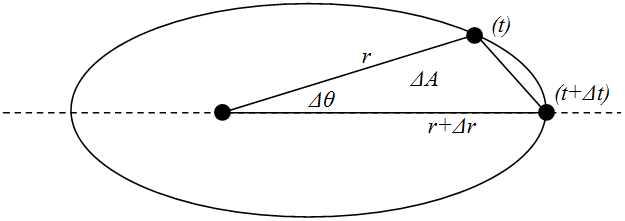
\includegraphics[scale=0.5]{elipse6.png}
    {\emph{\caption{Movimento orbital destacando dois pontos do movimento.}}}
    \label{fig6}
\end{figure}

Procuramos a área $\Delta A$ varrida por um corpo em seu movimento orbital, após uma passagem de tempo $\Delta t$ e uma variação angular $\Delta \theta$. Da figura 6, podemos obter que:

\begin{eqnarray}
	\Delta A = \frac{r(r+\Delta r)}{2}sen(\Delta \theta) + borda\label{eq53}
\end{eqnarray}

Tal borda corresponde à parte curva externa ao retângulo (que traz o primeiro termo à direita da equação anterior), e ela tende a zero quando a passagem de tempo também tende a zero. Acrescentando a variação angular e removendo o termo correspondente à borda (também bem pequeno em relação ao triângulo):

\[
	\Delta A = \frac{r(r+\Delta r)}{2}\left(\frac{sen(\Delta \theta)}{\Delta \theta}\right)\Delta \theta
\]

Dividindo tudo isso pelo tempo transcorrido:

\[
    \frac{\Delta A}{\Delta t} = \frac{r(r+\Delta r)}{2}\left(\frac{sen(\Delta \theta)}{\Delta \theta}\right)\frac{\Delta \theta}{\Delta t}
\]

Para descobrir a área transcorrida em função do tempo, é necessário avaliar o limite da expressão acima quando $\Delta t \rightarrow 0$, limite para o qual também ocorrem os limites $\Delta \theta \rightarrow 0$ e $\Delta r \rightarrow 0$:

\begin{eqnarray}
	 \lim_{\Delta t \rightarrow 0}\left({\frac{\Delta A}{\Delta t}}\right) = \frac{r^2}{2}\left(\lim_{\Delta \theta \rightarrow 0}{\frac{sen(\Delta \theta)}{\Delta \theta}}\right)\left(\lim_{\Delta t \rightarrow 0}{\frac{\Delta \theta}{\Delta t}}\right) + \frac{r}{2}\left(\lim_{\Delta \theta \rightarrow 0}{\frac{sen(\Delta \theta)}{\Delta \theta}}\right)\left(\lim_{\Delta t \rightarrow 0}{\frac{\Delta \theta}{\Delta t}}\right)\left(\lim_{\Delta r \rightarrow 0}{\Delta r}\right) \label{eq54}
\end{eqnarray}

É fácil de ver que o segundo termo da soma à direita vai a zero, pois $\lim_{\Delta r \rightarrow 0}{\Delta r} = 0$. Os demais limites presentes trazem:

\[
	\lim_{\Delta t \rightarrow 0}{\frac{sen(\Delta \theta)}{\Delta \theta}} = 1
\]

\[
	\lim_{\Delta t \rightarrow 0}{\frac{\Delta \theta}{\Delta t}} = \dot{\theta}
\]

Logo:

\[
	\lim_{\Delta t \rightarrow 0}\left({\frac{\Delta A}{\Delta t}}\right) = \frac{dA}{dt} = \frac{r^2\dot{\theta}}{2}
\]

Esta expressão ainda não nos ajuda completamente. No entanto, se multiplicarmos e dividirmos pela massa \textit{m} do corpo, retomamos a expressão do momento angular no numerador à esquerda. Como ele é constante:

\begin{eqnarray}
	\frac{dA}{dt} = \frac{mr^2\dot{\theta}}{2m} = \frac{L}{2m} = constante \label{eq55}
\end{eqnarray}

Enfim provamos a 2ª Lei de Kepler, escrita inicialmente para planetas:{\\}{\\}
\textbf{\Large{2ª Lei de Kepler: a área varrida pelo vetor que liga um planeta ao Sol num dado intervalo de tempo é constante.}} {\\}

\section{3ª Lei de Kepler}

A última das leis de Kepler é, na verdade, uma consequência direta da lei anterior. O movimento dos planetas, dada a simetria de seu movimento, é periódico. Se este período tiver valor \textit{T}, da 2ª Lei:

\begin{eqnarray}
	\frac{dA}{dt} = \frac{L}{2m} = \frac{\text{Área da elipse}}{\text{Período}} = \frac{\pi ab}{T} \label{eq56}
\end{eqnarray}

Esta lei tem como objetivo trazer uma relação entre o período e o semi-eixo maior, logo não deve restar nem \textit{b} nem \textit{L} nesta equação. Para eliminarmos $b$, das fórmulas da elipse:

\[
	b = a\sqrt{1 - \epsilon^2}
\]

Com a fórmula da excentricidade da elipse, podemos escrever que:

\[
	1 - \epsilon^2 = 1 - \left(1 + \frac{2EL^2}{G^2M^2m^3}\right) = - \frac{2EL^2}{G^2M^2m^3}
\]

Mas, sendo a órbita elíptica:

\[
	E = -\frac{GMm}{2a}
\]

Logo:

\[
	1 - \epsilon^2 = -\frac{2L^2}{G^2M^2m^3}\left(-\frac{GMm}{2a}\right) = \frac{L^2}{GMm^2a} \rightarrow \sqrt{1-\epsilon^2} = \frac{L}{m}\sqrt{\frac{1}{GMa}}
\]{\\}

Com isso:

\[
	\frac{L}{2m} = \frac{\pi a^2}{T}\left(\frac{L}{m}\sqrt{\frac{1}{GMa}}\right)
\]{\\}

Simplificando:

\[
	\frac{1}{2} = \frac{\pi}{T}\left(\sqrt{\frac{a^3}{GM}}\right)
\]

Elevando os dois lados ao quadrado, podemos chegar, então, que:

\begin{eqnarray}
	\frac{a^3}{T^2} = \frac{GM}{4\pi^2} \label{eq57}
\end{eqnarray}

E esta expressão prova a última das leis de Kepler:{\\}{\\}
\textbf{\Large{3ª Lei de Kepler: a razao do cubo do semi-eixo maior com o quadrado do período orbital é constante para todos os corpos que orbitam o Sol.}} {\\}

Como a 3ª Lei desdobra da 2ª Lei, temos que apenas duas das leis de Kepler são teoricamente inéditas. No entanto, a 3ª Lei oferece um meio de se encontrar relações muito úteis das órbitas dos demais planetas e do próprio Sol (dado que a massa do corpo orbitado é a que aparece na equação), sendo por meio dos dados numéricos do movimento orbital dos planetas que Kepler chegou à esta relação. Seja como for, todas as três leis puderam ser provadas a partir de conceitos primordiais e de relações matemáticas envolvendo elipses.

\section{Análise gráfica do potencial efetivo}

Este tópico foi propositalmente deixado para o final para que todo o embasamento teórico das Leis de Kepler e a equação do movimento fossem deduzidos, para que o que fosse visualizado aqui não trouxesse maiores surpresas (e dado também que a prova das três leis de Kepler fluem melhor quando provadas conjuntamente).{\\}

Retomemos a expressão original do potencial efetivo $V_{eff}$:

\[
	V_{eff}(r) = \frac{L^2}{2mr^2} - \frac{GMm}{r} 
\]

Esta equação possui o mesmo formato gráfico que $(1/r^2 - 1/r)$, mostrado na fig. 7, a seguir. É possivel observar uma região negativa na qual existe uma tendência a $+\infty$ para $r \rightarrow 0_+$, um mínimo global numa região negativa, um ponto de inflexão e uma tendência a zero quando $r \rightarrow \infty$.

\begin{figure}[!htb]
    \centering
     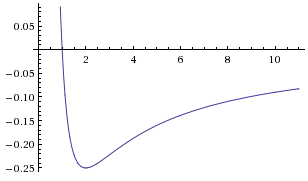
\includegraphics[scale=1]{elipse7.png}
    {\emph{\caption{Gráfico de $(1/r^2 - 1/r)$, trazido como exemplo de função de mesmo formato que $V_{eff}$.}}}
    \label{fig7}
\end{figure}

Se um corpo em órbita fechada está em uma posição $r$ extrema (se for um máximo, \textbf{apoastro}; se for um mínimo, \textbf{periastro}), então qualquer derivada de $r$ será nula, inclusive a temporal. Se retomarmos a expressão da energia E:

\[
	E = \frac{m\dot{r}^2}{2} + V_{eff}(r)
\]

Se estivermos numa posição extrema, então a energia total é dada somente por $V_{eff}$. Ou seja, se quisermos avaliar as posições extremas de uma determinada órbita, basta então traçar uma reta horizontal que cruze com o valor da energia total $E$ de uma órbita para descobrir os valores extremos do movimento. {\\}

Por exemplo, se $E$ for negativo, a órbita esperada será elíptica, e haverá dois pontos de cruzamento da curva de $V_{eff}$ com a reta $y=E$. Se $E$ for nulo, a órbita esperada será parabolica, e haverá um ponto de cruzamento visível entre a curva e a reta (o segundo ponto ocorrerá para $r \rightarrow \infty$. Se $E$ for positivo, então só haverá um ponto de cruzamento entre a curva e a reta (este único ponto corresponde à distância mínima que o corpo atinge durante todo o movimento antes de escapar da força gravitacional). {\\}

É possível verificar o comportamento gráfico de $V_{eff}$ ilustrado pelo gráfico anterior. Primeiramente, para $r \rightarrow 0_+$, o crescimento de $|V_{eff}|$ é muito grande, pois $1/r$ cresce muito rapidamente. No entanto, $1/r^2$ cresce ainda mais rápido, e portanto é o termo predominante. Logo, espera-se que $V_{eff}$ tenda a $+\infty$ para $r \rightarrow 0_+$.{\\}

No entanto, $V_{eff}$ possui um zero, o que faz com que passe para o lado negativo para valores de $r$ maiores que:

\begin{eqnarray}
	\frac{L^2}{2mr^2} - \frac{GMm}{r} = 0 \rightarrow r_0 = \frac{L^2}{2GMm^2}	\label{eq58}
\end{eqnarray} 

A partir de $r > r_0$, o termo que começa a majorar é o negativo, então a energia total é negativa. No entanto, como estes valores tendem a zero para $r \rightarrow \infty$, então a própria função deve chegar próxima deste limite para $r$ crescente. Isso traz um ponto de mínimo global para a função. Se derivarmos a expressão de $V_{eff}$ a procura de uma derivada nula:

\begin{eqnarray}
	\frac{dV_{eff}}{dr} = \frac{GMm}{r^2} -\frac{L^2}{mr^3} = 0 \rightarrow r_1 = \frac{L^2}{GMm^2} = 2r_0	\label{eq59}
\end{eqnarray} 

É possível verificar ainda um ponto de inflexão, encontrável a partir de:

\begin{eqnarray}
	\frac{d^2V_{eff}}{dr^2} = \frac{3L^2}{mr^4} - \frac{2GMm}{r^3}  = 0 \rightarrow r_2 = \frac{3L^2}{2GMm^2} = 3r_0	\label{eq60}
\end{eqnarray}

Para verificar quanto vale $r_0$, basta compararmos a expressão com aquela do \textit{semi-latus rectum} para órbitas, e verificar que:

\begin{eqnarray}
	l = 2r_0	\label{eq61}
\end{eqnarray}

Se a energia $E$ de um corpo é menor que a energia mínima do gráfico de $V_{eff}(r)$, isso nos traz que a energia cinética do corpo é negativa, o que é um absurdo. Se $E$ for exatamente o valor mínimo do gráfico, então apoastro e periastro terão a mesma distância, o que corresponde a uma circunferência (a qual possui um \textit{semi-latus rectum} igual ao raio de sua órbita). E assim seguem as deduções do gráfico de $V_{eff}$.

\end{document}